\documentclass{standalone}
\usepackage{pgfplots}
\pgfplotsset{compat=newest}
\usepackage{pgfplotstable}
\begin{document}
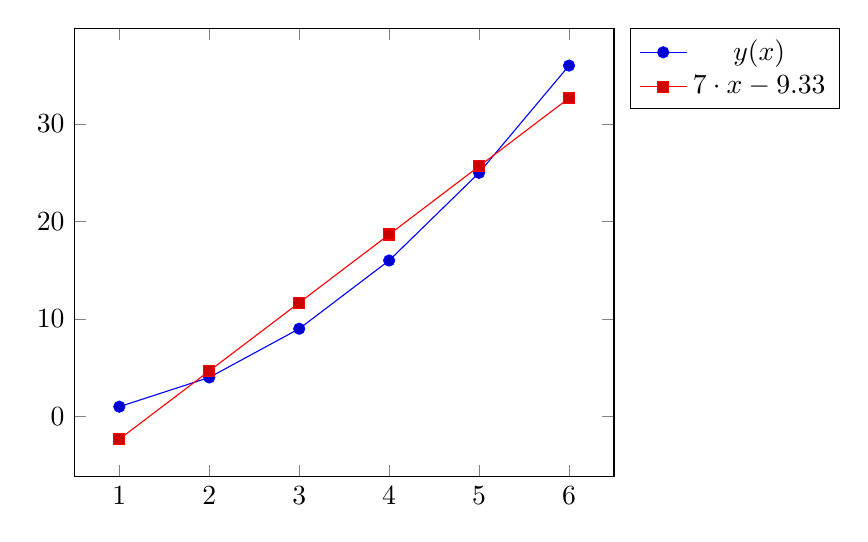
\begin{tikzpicture}
	\begin{axis}[legend pos=outer north east]
	\addplot table {% plot X versus Y. This is original data.
		X Y
		1 1 
		2 4
		3 9
		4 16
		5 25
		6 36
	};
	\addplot table[
		y={create col/linear regression={y=Y}}] % compute a linear regression from the input table
	{
		X Y
		1 1 
		2 4
		3 9
		4 16
		5 25
		6 36
	};
	%\xdef\slope{\pgfplotstableregressiona} %<-- might be handy occasionally
	\addlegendentry{$y(x)$}
	\addlegendentry{% 
		$\pgfmathprintnumber{\pgfplotstableregressiona} \cdot x  
		\pgfmathprintnumber[print sign]{\pgfplotstableregressionb}$}
	\end{axis}
\end{tikzpicture}
\end{document}
